\documentclass[12pt]{article}


\usepackage{amsmath}
\usepackage{amssymb}
\usepackage{attrib}
\usepackage{color}
\usepackage{fancyhdr}
\usepackage{graphicx}
\usepackage{hyperref}
\usepackage{makeidx}
\usepackage{stmaryrd}
\usepackage{xcolor}

\usepackage{preamble/lgarron-1.4.1}


\hypersetup{%
  colorlinks=true,% hyperlinks will be coloured
  linkcolor=blue,% hyperlink text will be green
  linkbordercolor=blue,% hyperlink border will be red
}

\def\rf{{\ \overset{R}\longleftarrow\ }}

\makeindex

\usepackage{multirow}

\usepackage{subfigure}

\usepackage{fancyhdr}
\pagestyle{fancy}
\fancyhead[C]{SPCS Cryptography -- Homework 10}
\rhead{}

\lhead{}



%%%%%%%%%%%%%%%%%%%%%%%%%%%%%%%%%%%%%%%%%%%%%%%%%%%%%%%%%%%%%%%%
  
\begin{document}

\section{Decryption}

Consider these handy diagrams from Wikipedia:

\begin{center}
\fbox{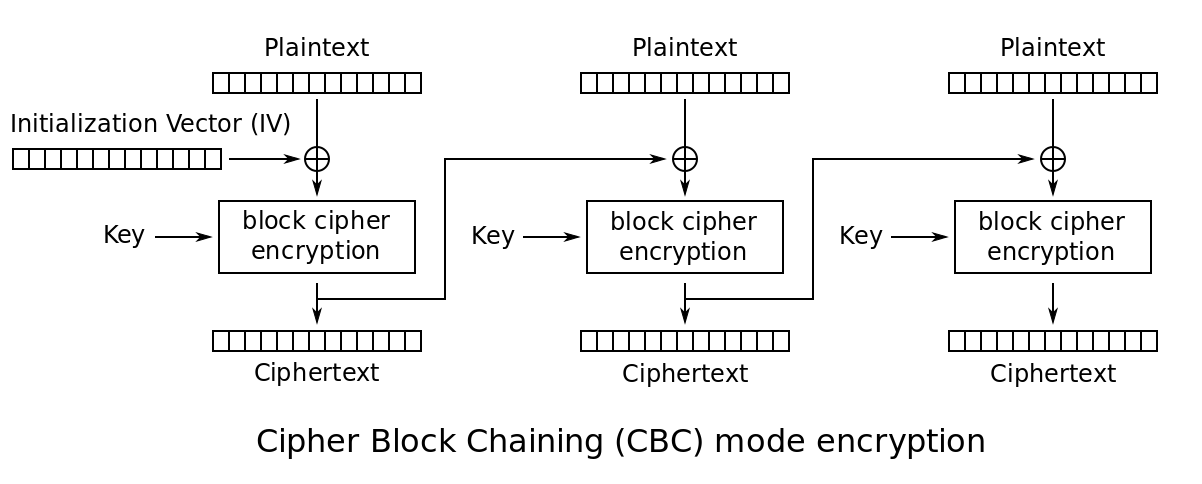
\includegraphics[width=10cm]{img/1202px-CBC_encryption.png}}\\
\fbox{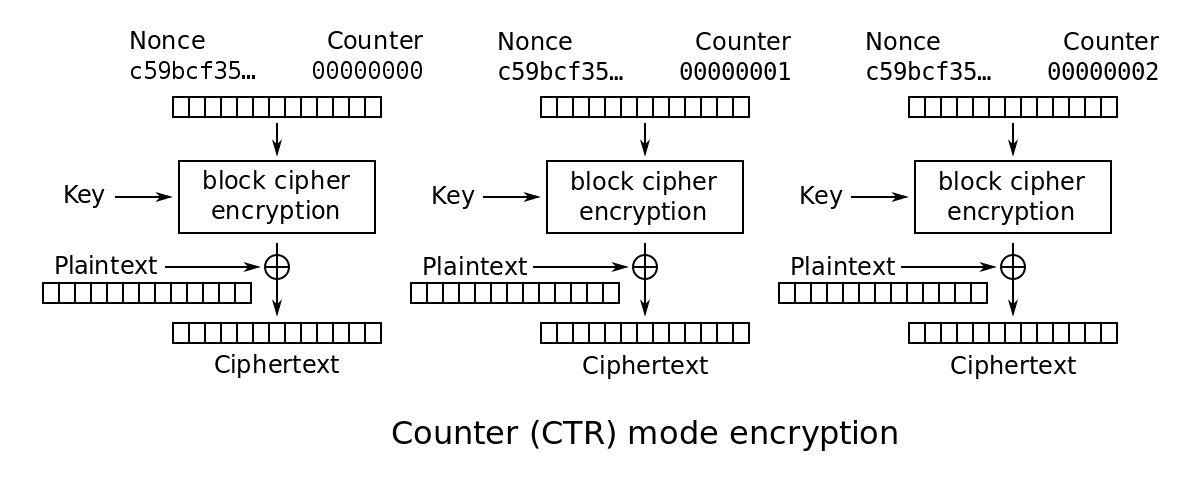
\includegraphics[width=10cm]{img/1202px-CTR_encryption_2.png}}\\
\fbox{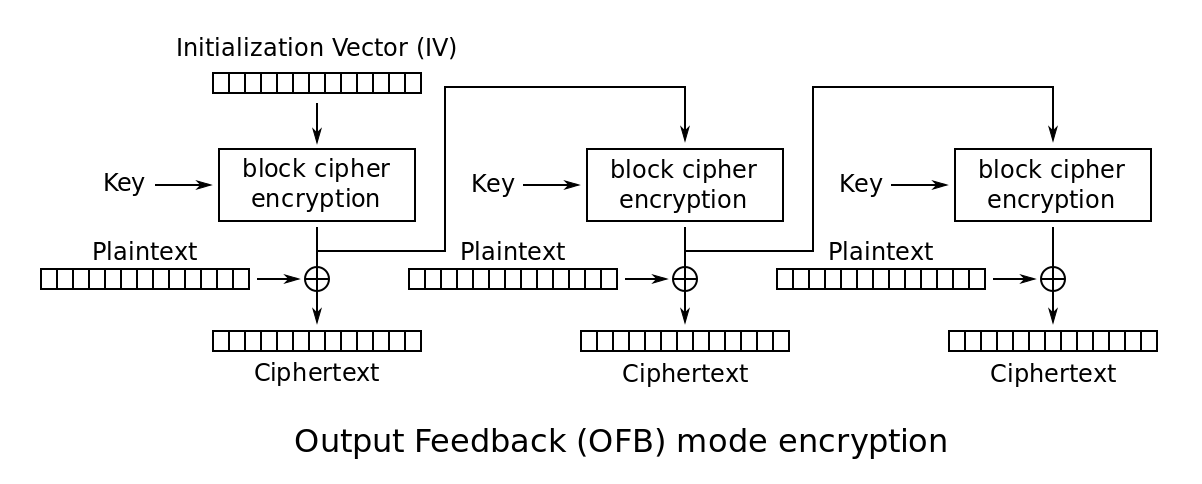
\includegraphics[width=10cm]{img/1202px-OFB_encryption.png}}
\end{center}

(CTR mode is a bit different from class because it considers the random part of the IV/nonce separate from the counter. Both of them are fairly similar, so feel free to use either version.)

\subsection{}

Draw the world's prettiest decryption diagrams for CTR, CBC, and CFB.


\section{}
Let $m$ be a message consisting of $k$ blocks (say $k = 100$). Alice encrypts $m$
using CBC mode and transmits the resulting ciphertext c to Bob. Due to a hardware error,
ciphertext block number $k/2$ is corrupted during transmission. All other ciphertext blocks
are transmitted and received correctly.

\begin{itemize}
\item Once Bob decrypts the received ciphertext, how many plaintext blocks will be corrupted?
\item Answer the same question for randomized counter mode.
\item Answer the same question for OFB mode.
\end{itemize}

(Don't just give a careless answer. Use your diagrams, and make sure can write a correct, written justification for your answer 

\section{}

Try to come up with your own block cipher.

Either break your system by showing an attack on semantic security, or try to show that it is secure if the PRF is secure.

(We haven't exactly defined how to do that, but you would start by showing that every input into a PRF is unique. That is, you never compute $E(k, a)$ for the same $k$ and $a$ in different places.)

\section{Nonce IV}

Suppose we choose the IV for counter mode as follows:

\begin{itemize}
\item The first $96$ bits are $\rf \{0, 1\}^{96}$
\item The final $32$ bits are all $0$.
\end{itemize}

For this problem, assume that every message $m$ has $|m| \leq 2^{32}$ (including padding; see problem \ref{padding}).

How many messages can we encrypt before we can break semantic security in the many-time CPA game?


CPA Security Game:
\begin{center}
\fbox{
\begin{tabular}{ccc}
& \tt{\bf EXP $b$} & \\
& & \\
\un{~~~~~~~~$\mathcal{C}$~~~~~~~~} & & \un{~~~$\mathcal{A}$~~~} \\
$k \rf \mathcal{K}$ & & \\
& $\longleftarrow$ & $m_0, m_1 \in \mathcal{M}$ (where $|m_0| = |m_1|$) \\
$E(k, m_b)$ & $\longrightarrow$ & (go back to last line for many-time) \\
& & $--------------$ \\
& &  b $\in \{0, 1\}$ \\
& & $\downarrow$
\end{tabular}
}
\end{center}




\newpage
\section{Padding}

\label{padding}

So far, we've only been able to encrypt messages that are a multiple of 128 bits (the AES block size).

We usually use a \emph{padding function} to turn every message into one that splits into blocks evenly. We can encrypt/decrypt that padded message, and remove the padding to get back the original message.

\subsection{}

Consider the following function $pad(m)$:

\begin{itemize}
\item Write $m$ in binary.
\item Add a $1$ at the end.
\item Add $0$ at the end until the message divides evenly into the block size.
\end{itemize}

\subsubsection{}

Write the function $unpad$ such that $unpad(pad(m)) = m$.

\subsubsection{}

How long is $pad(m)$ in terms of $|m|$?\\\\
(Recall: $|m|$ is the length of $m$. If $m\in \{0, 1\}^n$, then $|m| = n$.)

\subsubsection{}

Prove that every secure block padding scheme has at least one message $m$ whose padded version $pad(m)$ is at least one entire block longer.

\subsubsection{}

What properties must every padding scheme have?

\subsubsection{}
Try to come up with another padding scheme. Show that it works for any message in $\{0, 1\}^n$ (for any $n \in \Z$).

\subsection{}

Find a way to encrypt messages using OFB and CTR such that the resulting encryption is not any longer (apart from the IV).

\subsection{Ciphertext Stealing}

Don't try this until you've solved all the other problem:

Find a way to encrypt messages using CBC such that the resulting encryption is not any longer (apart from the IV).

(This one is very hard, and has a creative, non-obvious solution. It's really cool, though.)


\end{document}
